\documentclass[parskip]{scrartcl}
\usepackage[utf8]{inputenc}
\usepackage[ngerman]{babel}
\usepackage[round]{natbib}
\usepackage{color} % used for comments
\usepackage{listings}
\usepackage{url}
\usepackage{graphicx}
\graphicspath{ {img/} }
\lstset {
  language=xml,
  basicstyle={\footnotesize\ttfamily},
  numbers=none,
  aboveskip=5mm,
  belowskip=5mm,
  showstringspaces=false,
  columns=flexible,
  keywordstyle={\bfseries\color{blue}},
  commentstyle={\color{red}\textit},
  stringstyle=\color{magenta},
  frame=single,
  breaklines=true,
  breakatwhitespace=true,
  tabsize=4,
  morekeywords={rdf,rdfs,owl}  % <-- adding custom keywords
}

\linespread{1.2}

\begin{document}
\subject{Projektdokumentation im Modul Semantic Web}
\title{Verbreitung von Musik-Titeln nach deren Verwendung in einem Kinofilm}
\author{Patrick Bachmann}
\date{\today}

\maketitle


\paragraph{Recherchefragestellung: }
Welche Musik-Titel sind nach der Verwendung in einem Kinofilm in den Top 50 der Charts aufgetaucht?

\section{Inhaltliche Interpretation der Fragestellung}

Die Verwendung von Musik in Filmen ist ein gängiges Mittel um den gezeigten Bildern mehr Ausdruck zu verleihen und die Stimmung hervorzuheben. Neben der klassischen Filmmusik, welche individuell für den Film angefertigt wird, werden auch häufig kommerzielle Titel von Künstlern verschiedenster Stilrichtungen und Bekanntheitsgrade verwendet.

Die Fragestellung soll untersuchen, welche kommerziellen Musik-Titel nach der Verwendung in einem Kinofilm populär wurden bzw. erneut Popularität erreichten.

\pagebreak
\section{Relevante Datenquellen}

Für die Beantwortungen der Fragestellung werden folgende Daten benötigt:
\begin{itemize}
    \itemsep 1pt
    \parskip 0pt
    \parsep 0pt
    \item Kinofilme
    \begin{itemize}
            \item enthaltene Musiktitel
            \item Veröffentlichungsdatum
    \end{itemize}
        \item Charts
\end{itemize}

Nachfolgend sind die Datenquellen aufgelistet, welche benutzt wurden um diese Informationen zu akquirieren.

\subsection{Tunefind}
\label{subsec:tunefind}

Tunefind ist eine Community geführte Datenbank für Musik-Titel, welche in Serien und Kinofilmen Verwendung fanden.

\begin{tabular}{l|p{9cm}}
	Link & \url{http://www.tunefind.com/} \\
 	Datenformat & JSON \\
 	Schnittstelle & REST-Api \\
 	Lizenz & siehe \url{http://www.tunefind.com/api} \\
 	Open Data & $\star\star\star$ \\
\end{tabular}

\subsection{OMDb - The Open Movie Database}

Die Open Movie Database ist eine Web-Service, welcher eine Auswahl an Daten der IMDB über eine API zur Verfügung stellt. Es ist möglich einen Film über seinen  Titel oder seine IMDb ID zu finden. Die Suche über den Titel funktioniert dabei wie eine typische Suchfunktion und liefert auch bei verschiedenen Schreibweisen des Titels zuverlässig Ergebnisse.

\begin{tabular}{l|p{9cm}}
    Link & \url{http://www.omdbapi.com/} \\
    Datenformat & JSON, XML \\
    Schnittstelle & REST-API \\
    Lizenz & unbekannt \\
    Open Data & $\star\star\star$ \\
\end{tabular}

\subsection{IMDb}

Die Internet Movie Database ist die größte Datenbank für Filme, Serien und Spiele. Sie enthält eine Vielzahl von Informationen wie z.B. Regisseur, Schauspieler und die Veröffentlichungsdaten getrennt nach Ländern.

\begin{tabular}{l|p{9cm}}
	Link & \url{http://www.imdb.com/} \\
 	Datenformat & HTML \\
 	Schnittstelle & HTTP \\
 	Lizenz & unbekannt \\
 	Open Data & $\star\star$ \\
\end{tabular}

\subsection{Offizielle Charts}

Die Offiziellen Charts werden von der GfK zur Verfügung gestellt. Seit dem 02.01.1978 werden hier wöchentlich die Verkaufszahlen von Musik in Deutschland mit einem Ranking von 1 bis 100 bewertet. Dabei gilt es verschiedene Unterteilungen wie z.B. Single, Album und Compilation.

\begin{tabular}{l|p{9cm}}
    Link & \url{https://www.offiziellecharts.de} \\
    Datenformat & HTML \\
    Schnittstelle & HTTP \\
    Lizenz & unbekannt \\
    Open Data & $\star\star$ \\
\end{tabular}

\section{Extraktion relevanter Daten und import in einen Triplestore }

Die Extraktion der Daten wurde bei allen Datenquellen über Python-Skripte realisiert. Für jede Datenquelle wurde ein Skript mit zwei Phasen erstellt. Die \texttt{LoadFromWeb}-Phase lädt die Daten von der Datenquelle herunter und speichert sie als Textdatei mit JSON-Format ab. Die \texttt{ConvertToRdf}-Phase lädt die abgespeicherten Daten aus der vorher gespeicherten Datei und wandelt diese in Tripel um, welche im Turtle-Format abgespeichert werden. Die Phasen können kombiniert oder einzeln ausgeführt werden. Dafür muss dem Skript das Argument \texttt{-l} für die \texttt{LoadFromWeb}-Phase und \texttt{-r} für die \texttt{ConvertToRdf}-Phase mitgegeben werden.

Die erzeugten Dateien werden im Ordner \texttt{data/} abgelegt. Die Dateinamen sind im Kopfbereich des jeweiligen Skriptes festgeschrieben.


\subsection{Verwendete Bibliotheken}

\paragraph{HTML Extraktion}
Für die Extraktion von Daten aus HTML-Dateien wird die Bibliothek \texttt{beautifulsoup4  (v4.3.2)} verwendet. Sie ermöglicht ein einfaches arbeiten auf dem DOM-Baum.

\paragraph{RDF}
Für das Erstellen der Tripel sowie die Speicherung im Turtle-Format wird \texttt{rdflib (v4.2.0)} verwendet. 

\subsection{Extraktion Tunefind}

Tunefind stellt eine API bereit, welche die Daten der Webseite im JSON- oder XML-Format abrufbar macht. Für die Benutzung der API war eine Registrierung erforderlich. Anschließend konnte ein API Benutzernamen und ein API Passwort angefordert werden.
Um den Endpunkt von Tunefind erfolgreich anzusprechen, mussten einige Besonderheiten bzgl. des HTTP-Request-Headers beachtet werden. Es wurde ein Header in folgender Form benutzt:

\begin{lstlisting}[caption={HTTP-Request-Header}, label={list:httpHeader}]
accept: "text/html, application/json"
accept-encoding: "gzip, deflate"
authorization: "Basic %login%"
user-agent: "%appName%;%email%"
\end{lstlisting}

\begin{description}
    \item[accept] \hfill \\
        Gibt das erwartete Antwortformat an. Da JSON sich sehr gut mit Python verarbeiten lässt, wurde dieses Format gewählt.
    \item[accept-encoding] \hfill \\
        Gibt an, dass die Daten gzip-komprimiert erwartet werden.
    \item[authorization] \hfill \\
        Angaber der API-Login Daten für die HTTP-Basic-Authentication.
        Die Variable \texttt{\%login\%} wird mit dem base64-codierten Login-String bestehend aus API Benutzernamen und API Passwort ersetzt.
    \item[user-agent] \hfill \\
        Gibt an, welche Anwendung die Anfrage abgeschickt hat. Der Endpunkt von Tunefind lehnt jede Anfrage ab, welche diese Eigenschaft nicht mitschickt. Da es zum guten Ton gehört, wurde neben dem Anwendungsnamen auch eine E-Mail Adresse für die Kontaktaufnahme angegeben. 

\end{description}

Weiterhin ist der Endpunkt auf eine Anfrage pro Sekunde limitiert.

Die \texttt{LoadToRdf}-Phase und somit die Durchführung der Datenakquise beginnt mit einer Anfrage an:\\
\texttt{https://www.tunefind.com/api/v1/movie}

Das Ergebnis ist eine Liste mit allen in der Datenbank vorhandenen Filmen. Über die Id können nun die Details zu jedem Film abgerufen werden. Dies geschieht mit Anfragen an:\\
\texttt{https://www.tunefind.com/api/v1/movie/<movie-id>}

Diese Details enthalten unter anderem die Musik-Titel, welche zu dem angegeben Film in der Datenbank hinterlegt sind.
Es wird eine Liste mit allen verfügbaren Filmen und ihren Musik-Titeln erstellt. Das Ergebnis wird in folgendem JSON-Format abgespeichert:

\begin{lstlisting}[caption={Tunefind JSON-Format}, label={list:tunefindJson}]
[  
    {  
        "soundtrack":[  
            {
                "artist":"",
                "title":""
            },
        ...
        ],
        "title":""
    },
    ...
]
\end{lstlisting}

Die \texttt{ConvertToRdf}-Phase lädt die abgespeicherten Daten wieder und konvertiert sie in Tripel. Dazu wird folgendes Schema verwendet:

\begin{figure}[htbp]
    \centering
    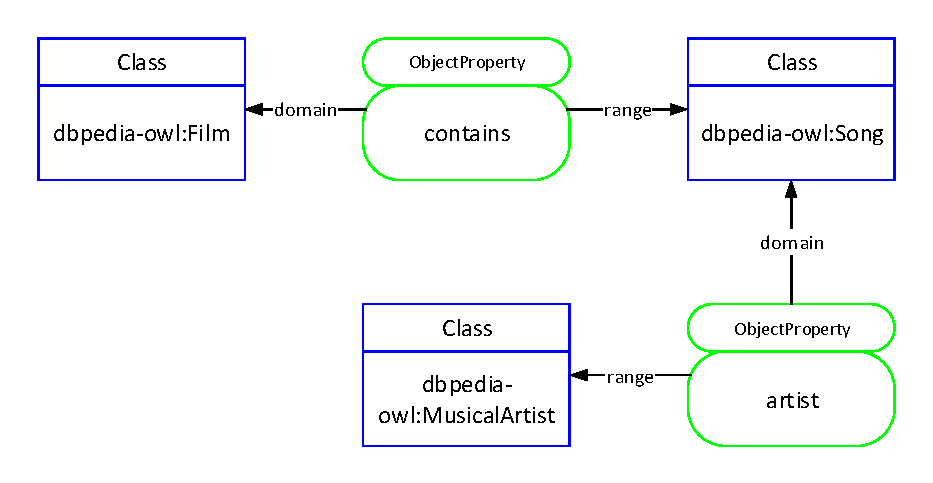
\includegraphics[scale=0.8]{tunefind}
\end{figure}

\subsection{Extraktion OMDb}

Das OMDb Projekt stellt über eine API Daten der IMDb bereit, da diese selbst keinen Endpunkt zur Verfügung stellt. Der Endpunkt der OMDb ist frei benutzbar und erfordert keine Registrierung oder einen API-Schlüssel.

Die Anfragen an die OMDb API bauen auf den Daten von Tunefind auf. Die Datei im JSON-Format, welche bei den Anfragen an Tunefind erstellt wurde, wird von dem Skript für die OMDb eingelesen. Mit den bereits akquirierten Filmtiteln wird nun der Endpunkt der OMDb-Api angefragt:\\
\texttt{http://www.omdbapi.com/?t=<Filmtitel>\&plot=short\&r=json}

Das Ergebnis sind die wichtigsten Informationen über den Film. Von Interesse ist dabei jedoch nur die ID der IMDb. Zusammen mit dem Filmtitel wird diese im JSON-Format abgespeichert.

\begin{lstlisting}[caption={OMDb JSON-Format}, label={list:omdbJson}]
[  
    {  
        "title":""
        "imdbid":""
    },
    ...
]
\end{lstlisting}

Eine Konvertierung in Tripel ist bei dieser Datenquelle nicht nötigt, da sie nur als Zwischenschritt zur Gewinnung der IMDb ID dient.

\subsection{Extraktion IMDb}

Die IMDb als größte Film- und Fernseh-Datenbank stellt von sich aus keinen Endpunkt zur Verfügung. Die Informationen, welche über die OMDb-Api gewonnen werden können sind nicht ausreichend, weshalb für die Akquirierung der benötigten Daten nun HTML-Seiten geparst werden müssen. Dafür werden die Daten der OMDb eingelesen und mithilfe der IMDb ID die Info-Seiten des Films aufgerufen.

Die Veröffentlichungsdaten für die Filme werden der \texttt{ReleaseInfo}-Seite entnommen:\\
\texttt{http://www.imdb.com/title/<ID>/releaseinfo}

Weiterhin wurden die Schauspieler und die Regisseure aus der \texttt{Cast}-Übersicht extrahiert:\\
\texttt{http://www.imdb.com/title/<ID>/fullcredits}

In der Konvertierungs-Phase wurden nun noch zusätzlich einige Einschränkungen hinzugefügt, um die Anzahl der erzeugten Tripel zu verringern (siehe PROBLEME). Es werden nur Filme übernommen, deren frühstes Veröffentlichungsdatum mindestens im Jahr 2005 liegt. Weiteren werden nur die Veröffentlichungsdaten von Deutschland, Großbritannien sowie den Vereinigten Staaten und die ersten zehn Schauspieler konvertiert.



\begin{figure}[htbp]
    \centering
    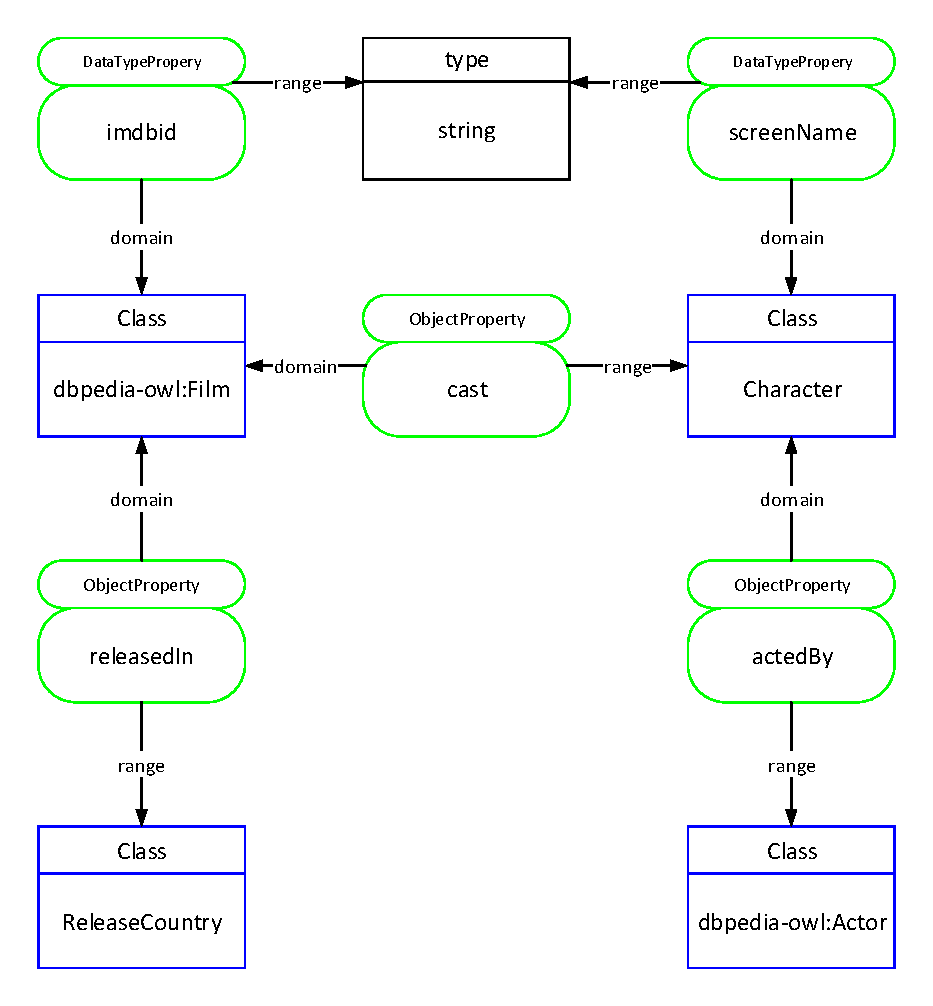
\includegraphics[scale=0.8]{imdb}
\end{figure}

\subsection{Extraktion Charts}

Wie auch die IMDb, stellen die Offizielen Charts keine API zur Verfügung. Weshalb auch hier auf die Daten aus den HTML-Seiten zurückgegriffen werden muss. Im Gegensatz zu der OMDb und der IMDb baut diese Datenquelle nicht auf Daten des jeweiligen Vorgängers auf. Sie ist somit eigenständig benutzbar.

Die Akquirierung der Daten erfolgt vom 01.01.2000 bis zum 31.05.2015. Da die Charts wöchentlich aktualisiert werden, wird folgende URL auch nur im Abstand von sieben Tagen aufgerufen:

\texttt{https://www.offiziellecharts.de/charts/single/for-date-<DATE>}

Für die Variable \texttt{<DATE>} wird das jeweilige Datum in Millisekunden eingesetzt. Von den Hundert Musiktiteln in den wöchentlichen Charts, werden nur die ersten 50 abgespeichert.

Die Konvertierung zu den Tripeln wurde bei diesem Skript nachträglich angepasst, da sich erst nach der Datenakquirierung dafür entschieden wurde, nur Filme ab dem Jahr 2005 zu betrachten. Es werden alle Charts vom 01.01.2005 bis zum 31.05.2015 als Tripel persistiert.


\subsection{Import in einen Triplestore}
Als Triplestore wurde Stardog verwendet. Er zeichnet sich durch eine einfache Handhabung und Konfiguration aus.

Es wurde versucht den Import der Tripel über die Python-Skripte zu realisieren. Jedoch wird für den Aufbau einer Verbindung über die „rdflib“ zu Stardog eine Abhängigkeit benötigt, welche unter Windows nicht auflösbar war. Deshalb wurden die Dateien mit den Tripel manuell über die Web-Oberfläche von Stardog importiert. Für jede Datenquelle zuvor eine eigene Datenbank angelegt.


\section{Verlinkung von Ressourcen}

Die Verlinkung erfolgt über die GND. dabei werden im Triple-Store \verb+owl:sameAs+ Triple\footnote{OWL Web Ontology Language
Reference owl:sameAs: \url{http://www.w3.org/TR/owl-ref/#sameAs-def}} hinzugefügt. Die Listing \ref{list:sameAs} zeit dies an einem Beispiel:

\begin{lstlisting}[caption={Beispiel für die Verwendung von owl:sameAS}, label={list:sameAs}]
http://catalogs-professorum.org/lipsiensis/Schuecking_144 owl:sameAs http://d-nb.info/gnd/117124931.
\end{lstlisting}


\textcolor{blue}{\textbf{Es handelt sich hier um ein Muster, das Dokument ist daher unvollständig...}}

\section{Anfrage an die Forschungswissensbasis}

\subsection{SPARQL-Anfrage}

\subsection{Ergebnis der Anfrage}


\textcolor{blue}{\textbf{Es handelt sich hier um ein Muster, das Dokument ist daher unvollständig...}}


\section{Interpretation und Zusammenfassung}

\textcolor{blue}{\textbf{Es handelt sich hier um ein Muster, das Dokument ist daher unvollständig...}}

\bibliographystyle{lnig.bst}
\bibliography{Projektdokumentation}



\end{document}
